\chapter{Podstawy teoretyczne i~przegląd rozwiązań}
\label{chap:theory}
Poniżej są przedstawione
podstawy teoretyczne sieci neuronowych,
dalej algorytmów genetycznych,
by następnie pokazać,
iż można te dwie
rzeczywistości połączyć.
Ostatecznie są omówione
poprzednie rozwiązania ewolucji
architektur sieci neuronowych.

\section{Sieć neuronowa}
Sieci neuronowe należą do grupy
matematycznych modeli obliczeniowych,
powstałych pod inspiracją sposobu funkcjonowania
procesów biologicznych w~układzie nerwowym.
Mają na celu znalezienie i~wykorzystanie
wysoko-poziomowych zależności
między danymi wejściowymi a~wyjściowymi,
które zostały dostarczone podczas procesu uczenia,
aby aproksymować odpowiedzi dla danych rzeczywistych.
Dzięki temu przeznaczeniu znalazły się
w~różnych obszarach takich jak:
klasyfikacja,
regresja, rozpoznawanie obrazów czy
przetwarzanie języka naturalnego%
\sscite{goodfellow2016deep}.

Podstawą działania sieci neuronowych
są sztuczne neurony.
W~najprostszej postaci sieci działanie
pojedynczego neuronu można
opisać następującym wzorem%
\sscite{haykin2009neural}:
$$
  y=f\left(
    \sum_{i=1}^{n}{w_i x_i}
    +b
  \right),
$$
gdzie:
\begin{nospitemize}
  \item $x_i$ -- wartości wejściowe neuronu,
  \item $w_i$ -- wagi połączeń,
  \item $b$ -- wyraz wolny,
  \item $f\left(\dots\right)$ -- funkcja aktywacji,
  \item $y$ -- wartość wyjściowa neuronu.
\end{nospitemize}
Oznacza to, że otrzymuje on zestaw wartości wejściowych,
które są mnożone przez odpowiadające im wagi,
a~następnie sumowane.
Do otrzymanej sumy dodawany
jest wyraz wolny (ang. \textit{bias}),
po czym wynik przekazywany jest
do funkcji aktywacji.
Funkcja ta wprowadza nieliniowość do modelu,
dzięki czemu sieć neuronowa
może odwzorowywać zależności,
których nie da się opisać
za pomocą prostych modeli liniowych.

Odwzorowaniem biologicznych synaps pomiędzy
neuronami są sztuczne synapsy
zwane połączeniami (ang. \textit{edges}).
Każde połączenie posiada przypisaną wagę
określającą siłę wpływu jednego neuronu na drugi.
Uczenie sieci neuronowej polega
na modyfikowaniu wspomnianych wag
na podstawie funkcji błędu,
co jest kontrolowane przez
współczynnik uczenia sieci,
tak by zminimalizować błąd
dla danych treningowych%
\sscite{goodfellow2016deep}.

Obecnie sieci neuronowe są intensywnie
rozwijanym działem informatyki.
Z~tego powodu powstało wiele ich typów,
z~których najczęściej stosowane można
podzielić na \gls{FNN} oraz rekurencyjne
(ang. \textit{recurrent neural networks}).
Do pierwszej grupy należą między innymi:
\gls{MLP},
\gls{CNN}
oraz transformatory (ang. \textit{transformers}).
Do drugiej grupy należą sieci RNN, LSTM i~GRU,
wykorzystywane przede wszystkim
do przetwarzania danych sekwencyjnych%
\sscite{
  goodfellow2016deep,
  rutkowski2009ai,
}.

Sieci składają się z~trzech segmentów:
wejściowego, przetwarzającego i~wyjściowego.
Odpowiadają one kolejno receptorom, mózgowi i~efektorom%
\sscite{haykin2009neural}.
W~jednokierunkowych sieciach neuronowych
informacje przepływają wyłącznie
od segmentu wejściowego do wyjściowego,
bez występowania cykli oraz sprzężeń zwrotnych.

W~perceptronie wielowarstwowym
segmenty sieci upraszczają się odpowiednio
do trzech podstawowych rodzajów warstw:
\begin{nospitemize}
  \item \textbf{warstwę wejściową}
    -- odpowiedzialną za przyjęcie danych wejściowych,
  \item \textbf{warstwy ukryte}
    -- odpowiedzialne za przetwarzanie informacji
    i~ekstrakcję cech,
  \item \textbf{warstwę wyjściową}
    -- generującą końcowy wynik działania sieci.
\end{nospitemize}
Oraz są one ułożone szeregowo w~następujący sposób:\\
\begin{tikzpicture}[>=Latex]
  % nodes
  \node (in) at (0,0) {we};
  \node (h1) at (1,0) {u};
  \node (dots) at (2,0) {$\cdots$};
  \node (hN) at (3,0) {u};
  \node (out) at (4,0) {wy};
  \node (where) at ($(5,-8pt)!2pt!(6,-8pt)$) {, gdzie:};

  % arrows
  \draw[->] (in)--(h1);
  \draw[->] (h1)--(dots);
  \draw[->] (dots)--(hN);
  \draw[->] (hN)--(out);

  % brace
  \coordinate (a) at (1,-5pt);
  \coordinate (b) at (3,-5pt);
  \draw[
    decorate,
    decoration={brace,mirror,amplitude=8pt},
  ] ($ (a)!-5pt!(b) $)--($ (b)!-5pt!(a) $) node[midway,below=8pt] {$n$};
\end{tikzpicture}
\begin{nospitemize}
  \item we -- warstwa wejściowa,
  \item u -- warstwa ukryta,
  \item wy -- warstwa wyjściowa,
  \item $n$ -- liczba warstw ukrytych.
  \item \raisebox{3pt}{\tikz[>=Latex]{
    \draw[->] (0,0)--(10pt,0)
  }} -- kierunek przetwarzania danych.
\end{nospitemize}
{\setlength{\parskip}{0pt}
Zatem wynik działania
każdego neuronu zależy jedynie
od wartości neuronów znajdujących się
w~poprzednich warstwach%
\sscite{goodfellow2016deep}.
}

Jest to charakterystyczne dla sieci \gls{MLP},
w~których połączenia występują tylko
pomiędzy sąsiadującymi warstwami, co powoduje,
iż każda warstwa przetwarza dane wyłącznie
dostarczone przez warstwę
bezpośrednio ją poprzedzającą.
Eliminuje to możliwość występowania
bezpośrednich połączeń pomiędzy warstwami
niesąsiadującymi ze sobą.
Co oznacza, iż obie sieci przedstawione
na \cref{fig:fnn_vs_mlp} są jednokierunkowe,
jednak tylko \textbf{\subref{subfig:fnn_mlp}} spełnia
definicję wielowarstwowego perceptronu%
\sscite{haykin2009neural}.
\begin{figure}
  \centering
  \subcaptionbox{\gls{FNN}\label{subfig:fnn}}{%
    \immediate\write18{sh ./img/drawio_to_pdf img/02_img/fnn/fnn.drawio}
    \includegraphics[trim={0 0 0 0}, height=6.5cm, clip]{img/02_img/fnn/fnn.drawio.pdf}
  }
  \hspace{2cm}
  \subcaptionbox{\gls{MLP}\label{subfig:fnn_mlp}}{%
    \immediate\write18{sh ./img/drawio_to_pdf img/02_img/fnn/fnn_mlp.drawio}
    \includegraphics[trim={0 0 0 0}, height=6.5cm, clip]{img/02_img/fnn/fnn_mlp.drawio.pdf}
  }
  \caption{
    Przedstawione dwie sieci neuronowe
    zawierające po jednej z~każdego rodzaju warstwy:
    wejściowa, ukryta oraz wyjściowa.
    Obie architektury mają po dwa wejścia
    i~jednym wyjściu, dodatkowo są w~pełni połączone
    między sąsiednimi warstwami.
    Jedyna różnica, to jedno
    połączenie międzywarstwowe
    od neurony wejściowego
    do wyjściowego, omijające
    warstwę ukrytą,
    w~sieci \textbf{\subref*{subfig:fnn}},
    które nie występuje
    w~\textbf{\subref*{subfig:fnn_mlp}}.
  }
  \label{fig:fnn_vs_mlp}
\end{figure}

Liczba neuronów w~warstwie wejściowej
odpowiada liczbie cech w~danych wejściowych.
W~zadaniach klasyfikacji liczba neuronów wyjściowych
często odpowiada liczbie klas
lub jest o~jeden większa,
by oznaczyć dane nie pasujące do żadnej kategorii,
natomiast w~zadaniach regresyjnych
liczba neuronów może zaczynać się od jednego,
w~zależności od liczby przewidywanych wartości.

Powyżej omawiane warstwy są z~reguły zdeterminowane
przez dane i~specyfikę problemu,
więc do optymalizacji zostają warstwy ukryte
które w~największym stopniu można zmieniać.
Z~tego powodu to one mają największy wpływ
na zdolności sieci.
To one decydują czy sieć będzie zdolna
do modelowania skomplikowanych zależności.
Dlatego ich konfiguracja jest kluczowym
obszarem optymalizacji.

Największy wpływ na proces uczenia \gls{MLP}
mają następujące parametry:
\begin{nospitemize}
  \item liczba warstw ukrytych,
  \item liczba neuronów w~poszczególnych warstwach,
  \item topologia połączeń pomiędzy neuronami,
  \item sposób inicjalizacji wag,
  \item parametry procesu uczenia.
\end{nospitemize}

Ich dobór ma bezpośredni skutek
w~zdolnościach sieci do generalizacji
oraz osiąganiu zadawalających wyników,
co zostało zobrazowane na
\cref{fig:fitting_under_over}.
Mniejsza sieć (\cref{subfig:underfitting})
może nie być w~stanie odwzorować zależności
występujących w~danych (ang. \textit{underfitting}).
Z~kolei zbyt rozbudowana architektura
(\cref{subfig:overfitting}) powoduje dłuższe uczenie
i~działanie modelu oraz może prowadzić
do dopasowania się do zależności występujących
tylko w~danych treningowych (ang. \textit{overfitting}),
co spowoduje nie adekwatne odpowiedzi
dla danych uprzednio nieznanych.
Dlatego ważne jest dobranie sieci
o~odpowiedniej złożoności
(\cref{subfig:appropriate_capacity}),
gdyż przy nich istnieje
największe prawdopodobieństwo,
że będą po nauczeniu zdolne
do zadawalającej generalizacji.

\begin{figure}
  \centering
  \begin{subfigure}{0.3\textwidth}
    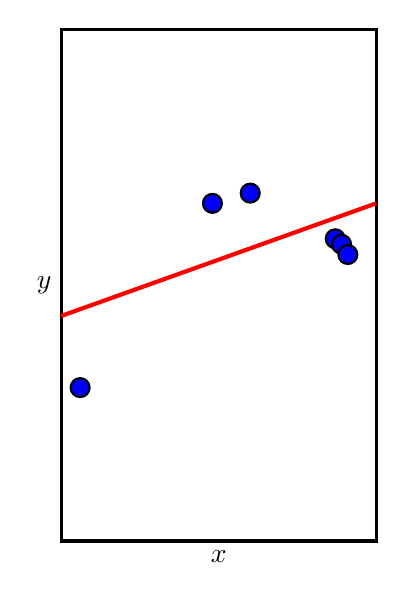
\begin{tikzpicture}
  \tikzset{
  data_pic/.pic={
    % plot frame
    \draw[line width=1.2pt] (0,0) rectangle (4,6.5);

    % data points
    \filldraw[blue, draw=black, line width=0.8pt] (0.24,1.95) circle (0.12);
    \filldraw[blue, draw=black, line width=0.8pt] (1.92,4.29) circle (0.12);
    \filldraw[blue, draw=black, line width=0.8pt] (2.40,4.42) circle (0.12);
    \filldraw[blue, draw=black, line width=0.8pt] (3.48,3.84) circle (0.12);
    \filldraw[blue, draw=black, line width=0.8pt] (3.56,3.77) circle (0.12);
    \filldraw[blue, draw=black, line width=0.8pt] (3.64,3.64) circle (0.12);

    % characteristic coordinates of plot
    \coordinate (-oo) at (0, 0);
    \coordinate (-top) at (2, 6.5);
    \coordinate (-bottom) at (2, 0);
    \coordinate (-left) at (0, 3.25);
  }
}

  % img
  \pic (pic_u) at (0, 0) {data_pic};
  \begin{scope}[shift={(pic_u-oo)}]
    \draw[red, line width=1.5pt]
      (0,2.86) -- (4,4.29);
  \end{scope}

  % % titles
  % \draw (pic_u-top) node[anchor=south] {Zbyt prosty model};

  % axis
  \draw (pic_u-bottom) node[anchor=north] {$x$};
  \draw (pic_u-left) node[anchor=east] {$y$};
\end{tikzpicture}
    \caption{Zbyt prosty model}
    \label{subfig:underfitting}
  \end{subfigure}
  \hfill
  \begin{subfigure}{0.3\textwidth}
    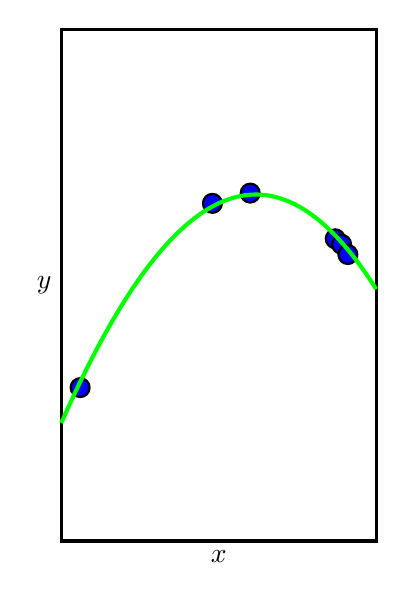
\begin{tikzpicture}
  \tikzset{
  data_pic/.pic={
    % plot frame
    \draw[line width=1.2pt] (0,0) rectangle (4,6.5);

    % data points
    \filldraw[blue, draw=black, line width=0.8pt] (0.24,1.95) circle (0.12);
    \filldraw[blue, draw=black, line width=0.8pt] (1.92,4.29) circle (0.12);
    \filldraw[blue, draw=black, line width=0.8pt] (2.40,4.42) circle (0.12);
    \filldraw[blue, draw=black, line width=0.8pt] (3.48,3.84) circle (0.12);
    \filldraw[blue, draw=black, line width=0.8pt] (3.56,3.77) circle (0.12);
    \filldraw[blue, draw=black, line width=0.8pt] (3.64,3.64) circle (0.12);

    % characteristic coordinates of plot
    \coordinate (-oo) at (0, 0);
    \coordinate (-top) at (2, 6.5);
    \coordinate (-bottom) at (2, 0);
    \coordinate (-left) at (0, 3.25);
  }
}

  % img
  \pic (pic_a) at (5.5, 0) {data_pic};
  \begin{scope}[shift={(pic_a-oo)}]
    \draw[green, line width=1.5pt]
      (0,1.5)
      .. controls (1.5,4.9) and (2.8,5.1) ..
      (4,3.2);
  \end{scope}

  % % titles
  % \draw (pic_a-top) node[anchor=south] {Odpowiedni model};

  % axis
  \draw (pic_a-bottom) node[anchor=north] {$x$};
  \draw (pic_a-left) node[anchor=east] {$y$};
\end{tikzpicture}
    \caption{Odpowiedni model}
    \label{subfig:appropriate_capacity}
  \end{subfigure}
  \hfill
  \begin{subfigure}{0.3\textwidth}
    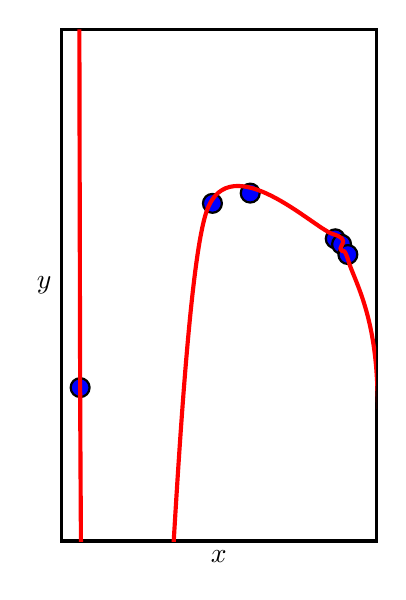
\begin{tikzpicture}
  \tikzset{
  data_pic/.pic={
    % plot frame
    \draw[line width=1.2pt] (0,0) rectangle (4,6.5);

    % data points
    \filldraw[blue, draw=black, line width=0.8pt] (0.24,1.95) circle (0.12);
    \filldraw[blue, draw=black, line width=0.8pt] (1.92,4.29) circle (0.12);
    \filldraw[blue, draw=black, line width=0.8pt] (2.40,4.42) circle (0.12);
    \filldraw[blue, draw=black, line width=0.8pt] (3.48,3.84) circle (0.12);
    \filldraw[blue, draw=black, line width=0.8pt] (3.56,3.77) circle (0.12);
    \filldraw[blue, draw=black, line width=0.8pt] (3.64,3.64) circle (0.12);

    % characteristic coordinates of plot
    \coordinate (-oo) at (0, 0);
    \coordinate (-top) at (2, 6.5);
    \coordinate (-bottom) at (2, 0);
    \coordinate (-left) at (0, 3.25);
  }
}

  % img
  \pic (pic_o) at (11, 0) {data_pic};
  \begin{scope}[shift={(pic_o-oo)}]
    \clip (0,0) rectangle (4,6.5);
    \draw[
      red,
      line width=1.5pt
    ] plot[smooth] coordinates {
      (0.23,6.5)
      (0.24,2.0)
      (0.25,0.0)
      (0.26,-2.0)
      (1.30,-0.1)
      (1.30,-2.0)
      (1.85,4.2)
      (3.45,3.90)
      (3.55,3.70)
      (3.65,3.55)
      (4.00,2.2)
      (4.10,-2.0)
    };
  \end{scope}

  % % titles
  % \draw (pic_o-top) node[anchor=south] {Zbyt złożony model};

  % axis
  \draw (pic_o-bottom) node[anchor=north] {$x$};
  \draw (pic_o-left) node[anchor=east] {$y$};
\end{tikzpicture}
    \caption{Zbyt złożony model}
    \label{subfig:overfitting}
  \end{subfigure}

  \caption{
    Trzy płaszczyzny
    z~\citebook[cite={rys. 5.2}]{goodfellow2016deep}
    ukazujące możliwe zachowania dla modeli:
    \textbf{\subref*{subfig:underfitting}}
    zbyt prostych w~stosunku do danych,
    \textbf{\subref*{subfig:overfitting}}
    zbyt złożonych oraz
    \textbf{\subref*{subfig:appropriate_capacity}}
    sieci o~złożoności odpowiadającej
    tej występującej w~danych.
    Punkty to przykładowe dane treningowe,
    a~linie (czerwone i~zielone),
    to przykładowe odpowiedzi modeli
    po nauczeniu sieci.
  }
  \label{fig:fitting_under_over}
\end{figure}

\toclesslabel\subsection{Architektura sieci neuronowej}{subsec:nn_architecture_theory}
Architektura sieci neuronowej określa
ułożenie i~typy neuronów oraz ich połączeń.
Jest ona jednym z~najważniejszych czynników,
które mają wpływ na zdolności modelu do:
aproksymacji funkcji,
szybkość uczenia i~odpowiedzi
oraz generalizacji wiedzy na nowe dane%
\sscite{haykin2009neural}.

Pojęcie architektury sieci w~literaturze
obejmuje funkcje aktywacji, rozłożenie neuronów
oraz połączenia między nimi%
\sscite{yao1999evolving}.

Przekładając powyższe na \gls{MLP}, architektura
odnosi się do funkcji aktywacji, liczby warstw,
neuronów w~nich i~połączeń.
W~niniejszej pracy rozważane
są wyłącznie \gls{pMLP}.
Oznacza to, że każda warstwa jest
w~pełni połączona z~warstwą następną,
więc sposób połączenia neuronów jest
z~góry ustalony i~nie podlega optymalizacji.
Z~tego powodu liczba połączeń nie stanowi
niezależnego parametru architektury,
lecz wynika bezpośrednio z~liczby neuronów
znajdujących się w~sąsiednich warstwach.
Zatem architektura sieci neuronowej
rozumiana będzie wyłącznie jako:
\begin{nospitemize}
  \item liczba warstw ukrytych,
  \item liczba neuronów w~każdej warstwie ukrytej,
  \item funkcja aktywacji zastosowana w~każdej warstwie.
\end{nospitemize}

Do architektury nie będą natomiast zaliczane
wartości wag i~wyrazów wolnych neuronów,
ponieważ są one wyznaczane podczas procesu uczenia.
Nie będą do niej również zaliczane parametry procesu
uczenia, takie jak współczynnik uczenia,
liczba epok czy zastosowany optymalizator.
Parametry te wpływają na przebieg uczenia,
lecz nie zmieniają struktury modelu.

Dobór odpowiedniej architektury
jest jednym z~najważniejszych zagadnień
podczas tworzenia sieci.
W~przypadku wybierania takiej architektury 
liczba parametrów jest znacząca.
Z~tego powodu można wykorzystać metody
automatycznej optymalizacji, które są przeznaczone
do przeszukiwania dużych przestrzeni rozwiązań%
\sscite{
  yao1999evolving,
  domashova2021optimal,
}.

\section{Algorytmy genetyczne}
Algorytmy genetyczne należą do grupy
algorytmów inspirowanych biologiczną ewolucją.
Algorytmy ewolucyjne opierają się na założeniu,
iż ewolucja, a~więc krzyżownie, mutacja
oraz naturalna selekcja, powoduje dążenie
do coraz większej optymalności w~populacji%
\sscite{
  goldberg1989genetic,
  eiben2015evolutionary,
}.

Algorytmy te zawierają więc
w~sobie populację osobników,
na których będą wykonywane operacje.
Osobniki przedstawiają potencjalne
rozwiązania, które określa się jako fenotyp.
Każdy z~osobników posiada swój kod genetyczny
(genotyp), którego części są przekazywane
osobnikom potomnym podczas krzyżowania
i~z~niego odkodowywana jest postać fenotypu.
Po odkodowaniu rozwiązania jest ono
oceniane przez algorytm%
\sscite{goldberg1989genetic}.

Ich jakość jest określana
za pomocą funkcji przystosowania
(ang. \textit{fitness function}).
Funkcja ta zwraca dla fenotypu danego osobnika
jego dostosowanie do środowiska.
Gdzie środowisko jest kryteriami optymalizacji,
które rozwiązania mają spełniać.
Im większa wartość zostanie zwrócona,
tym większe prawdopodobieństwo
będzie miał dany osobnik
dla przekazania cech
do następnych pokoleń%
\sscite{goldberg1989genetic}.

Klasyczny przebieg algorytmu genetycznego
przedstawia \cref{fig:genetic_flow},
którego szczególne elementy są omawiane
w~poniższych podrozdziałach.
\begin{figure}
  \centering
  \resizebox{.95\textwidth}{!}{%
    \begin{tikzpicture}[
  font=\sffamily\small,
  node distance=8mm and 8mm,
  >=Latex,
  arrow/.style={
    -{Latex[length=3mm,width=2mm]},
    thick,
    draw=gray!75,
  },
  process/.style={
    rectangle,
    draw=blue!60!black,
    % draw=gray!60!black,
    very thick,
    fill=blue!8,
    % fill=gray!8,
    align=center,
    text width=36mm,
    minimum height=10mm,
    inner xsep=3mm,
    inner ysep=2mm,
  },
  terminator/.style={
    rectangle,
    rounded corners,
    draw=green!45!black,
    % draw=gray!45!black,
    very thick,
    fill=green!10,
    % fill=gray!10,
    align=center,
    minimum width=24mm,
    minimum height=10mm,
    inner xsep=4mm,
    inner ysep=2mm,
  },
  decision/.style={
    diamond,
    aspect=2.15,
    draw=orange!70!black,
    % draw=gray!70!black,
    very thick,
    fill=orange!12,
    % fill=gray!12,
    align=center,
    text width=32mm,
    inner xsep=1mm,
    inner ysep=1mm,
  },
  label/.style={
    font=\sffamily\footnotesize,
    fill=white,
    inner sep=1.5pt,
    text=gray!20!black,
  },
]
  % nodes
  \node[process] (B) {Wygenerowanie początkowej populacji osobników};
  \node[decision, right=of B] (D) {Czy spełnione warunki końcowe?};
  \node[terminator, above=of D] (J) {Koniec};
  \node[terminator] (A) at (B |- J) {Początek};

  \node[process, right=of D] (I) {Wybranie osobników do następnej generacji};

  \node[process, below=of D] (E) {Wykonanie selekcji rodziców};

  \node[process, below=of E] (F) {Wykonanie krzyżowania rodziców};
  \node[process] (G) at (F -| I) {Wykonanie mutacji dzieci};
  \node[process] (H) at ($(G.north)!0.5!(I.south)$) {Wyliczenie przystosowania wszystkich nowych osobników};
  \node[process, anchor=south west] (C) at (B.west |- H.south) {Wyliczenie przystosowania każdego z~osobników};

  % edges
  \draw[arrow] (A) -- (B);
  \draw[arrow] (B) -- (C);
  \draw[arrow] (C.east) -| ($ (C.east)!0.5!(D.west)-(1.5mm,0) $) |- (D.west);

  \draw[arrow] (D) -- node[label, right=1pt, yshift=-1.5mm] {Tak} (J);
  \draw[arrow] (D) -- node[label, right=1pt, yshift=1.5mm] {Nie} (E);

  \draw[arrow] (E) -- (F);
  \draw[arrow] (F) -- (G);
  \draw[arrow] (G) -- (H);
  \draw[arrow] (H) -- (I);
  \draw[arrow] (I) -- (D);
\end{tikzpicture}%
  }
  \caption{
    Klasyczny przebieg algorytmu genetycznego
    opisany w~\citebook{eiben2015evolutionary}.
    Na początku generowana jest początkowa populacja,
    dla której osobników następnie
    są wyliczane przystosowania.
    Następnie występuje sprawdzenie
    spełnienia warunków końcowych,
    jeżeli zostały wypełnione
    to algorytm kończy swoje działanie,
    a~w~przeciwnym wypadku są wykonywane:
    selekcja, krzyżowanie, mutacja,
    wyliczenie przystosowania nowych osobników,
    wybranie następnej generacji,
    potem następuje powrót
    do sprawdzenia warunków końcowych.
  }
  \label{fig:genetic_flow}
\end{figure}

\tocless\subsection{Selekcja}
Selekcja jest procesem odpowiadającym
biologicznej selekcji naturalnej,
polegającym na wyborze bardziej
przystosowanych osobników,
by z~nich mogło powstać
następne pokolenie.
Dobra selekcja faworyzuje
lepiej przystosowane jednostki,
jednocześnie zachowując
różnorodność genetyczną.
Chcąc osiągnąć ten balans
powstało wiele metod selekcji,
są to między innymi selekcja ruletkowa,
turniejowa oraz rankingowa%
\sscite{goldberg1989genetic}.

\tocless\subsection{Krzyżowanie}
Krzyżowanie odwzorowuje biologiczne mieszanie
genów rodziców przy rozmnażaniu płciowym,
w~którym dziecko dostaje część genów
od jednego rodzica, a~część -- od drugiego.
Dzięki temu procesowi tworzone są nowe osobniki
posiadające cechy odziedziczone po rodzicach.
Sposób krzyżowania zależy od reprezentacji genotypu
i~są to między innymi:
krzyżowanie jedno- lub wielopunktowe,
równomierne oraz operatory przeznaczone
dla struktur o~zmiennej długości%
\sscite{
  goldberg1989genetic,
  stanley2002neat,
}.

\tocless\subsection{Mutacja}
Kolejnym elementarnym działaniem
w~algorytmach genetycznych jest mutacja.
Polega ona na losowej modyfikacji genotypu.
Podobnie jak w~przypadku krzyżowania
sposób wykonania tej czynności zależy
od reprezentacji genotypu,
może to być między innymi:
zmiana wartości pojedyńczego genu,
zmiana miejsc elementów w~genotypie
lub dodanie albo usuwanie
fragmentów kodu.
Celem tych działań jest
wprowadzanie do populacji
nowej informacji genetycznej
oraz zapobieganie przedwczesnemu zbieganiu
do lokalnych ekstremów optymalizacji%
\sscite{goldberg1989genetic}.

\tocless\subsection{Elitaryzm}
W~wielu implementacjach algorytmów genetycznych
stosowany jest elitaryzm.
W~przypadku jego zastosowania przenosi się
najbardziej przystosowanych osobników
do kolejnego pokolenia bez zmian
w~ich genotypie.
Takie rozwiązanie pozwala
uniknąć utraty najlepszych
ze znalezionych rozwiązań%
\sscite{eiben2015evolutionary}.

\tocless\subsection{Zastosowanie do optymalizacji}
Algorytmy genetyczne wykorzystuje się
w~poszukiwaniach optymalnego rozwiązania,
które byłyby trudne do rozwiązania
metodami analitycznymi.
Dobrze się sprawdzają w~przeszukiwaniu
dużych przestrzeni poszukiwań,
w~których występuje wiele lokalnych ekstremów
oraz nieciągłości funkcji celu.
Dzięki tym zdolnością są wykorzystywane
między innymi do:
projektowania konstrukcji,
planowania i~harmonogramowania zadań,
problemów logistycznych czy kombinatorycznych,
doboru cech i~strojenia
hiperparametrów w~uczeniu maszynowym,
oraz optymalizacji parametrów modeli i~systemów%
\sscite{eiben2015evolutionary}.

\section{Ewolucyjna optymalizacja sieci neuronowych}
Jak już zostało przytoczone
w~\cref{subsec:nn_architecture_theory}
architektura sieci jest jednym z~najważniejszych
elementów wpływającym na efektywność uczenia,
jak i~na jej późniejsze zdolności do realizacji zadań.
W~praktyce proces ten często opiera się
na wiedzy eksperckiej,
wcześniejszych doświadczeniach
oraz metodzie prób i~błędów.
A~wraz ze wzrostem liczby parametrów architektury,
takich jak liczba neuronów
czy rodzaje funkcji aktywacji
w~poszczególnych warstwach,
liczba możliwych konfiguracji rośnie bardzo szybko.
Powoduje to, że ręczne przeszukiwanie przestrzeni
rozwiązań staje się czasochłonne, a~nie gwarantuje
znalezienia optymalnego rozwiązania%
\sscite{
  goodfellow2016deep,
  yao1999evolving,
}.

W~celu automatyzacji tego procesu
można wykorzystać algorytmy ewolucyjne,
takie jak algorytmy genetyczne.
W~literaturze podejście to
widnieje pod nazwą neuroewolucji
(ang. \textit{neuroevolution}),
które w~ogólnym rozumieniu może odnosić się
do optymalizacji dowolnej części sieci,
ponieważ algorytm może
przeszukiwać przestrzeń rozwiązań
wyłącznie dla wartości wag,
architektury sieci
lub obu tych elementów jednocześnie%
\sscite{
  yao1999evolving,
  stanley2019neuroevolution,
}.

W~przypadku optymalizowania architektury sieci,
osobniki zawierają w~genotypie
zakodowany opis tej stuktury.
Więc w~zależności od typu budowanego modelu
oraz założeń danej problematyki zapisane
będą informacje umożliwiające skonstruowanie go.
Przykładowo w~\citebook[cite={481}]{miller1989designing}
zostaje przedstawiony opis zawierający
połączenia między neuronami
ze stałą liczbą neuronów.
Natomiast w~\citebook[cite={268}]{domashova2021optimal}
w~genotypie zawarta jest informacja
o~liczbie warstw, typach funkcji aktywacji
i~liczbie neuronów w~nich.

Ocena jakości osobników w~kontekście
sieci neuronowych powoduje,
że funkcja przystosowania jest związana
z~miarami jakości działania modelu.
Mogą być nimi w~zależności od typu problematyki:
dokładność klasyfikacji, wartość funkcji straty
lub inne tego rodzaju wskaźniki%
\sscite{
  goldberg1989genetic,
  yao1999evolving,
  eiben2015evolutionary,
}.

Badania nad wykorzystaniem algorytmów genetycznych
do projektowania sieci neuronowych prowadzone są
od końca lat osiemdziesiątych XX wieku.
Jedne z~pierwszych prac dotyczących tego zagadnienia
zostały przedstawione w~\citebook{miller1989designing},
gdzie autorzy wykorzystali algorytmy genetyczne
do automatycznego projektowania
połączeń między ustaloną liczbą neuronów.
W~kolejnych latach rozwijano zarówno metody
optymalizacji parametrów architektury,
jak i~podejścia umożliwiające ewolucję
całej struktury neuronowej.
Przykładem takiego rozwiązania jest algorytm NEAT
(\textit{NeuroEvolution of Augmenting Topologies}),
w~którym architektura sieci
może być stopniowo rozwijana
w~trakcie procesu ewolucyjnego%
\sscite{stanley2002neat}.
W~niniejszej pracy rozważany jest
bardziej ograniczony wariant tego problemu,
ponieważ analizowane są wyłącznie
w~pełni połączone wielowarstwowe perceptrony.
Oznacza to, że sposób połączenia neuronów
pomiędzy kolejnymi warstwami jest z~góry
ustalony i~nie podlega optymalizacji.
Zmianom podlega natomiast liczba warstw ukrytych,
liczba neuronów w~poszczególnych warstwach
oraz zastosowane funkcje aktywacji.

Metody neuroewolucji są wciąż
rozwijane i~wykorzystywane.
Znajdują zastosowanie, zwłaszcza
gdy przy danej problematyce
występuje duża liczba możliwych konfiguracji.
Przykłady współczesnych badań pokazują,
iż algorytmy genetyczne mogą
wspomagać proces poszukiwania
architektury osiągając
zadawalającą jakość działania
dla określonych problemów%
\sscite{
  domashova2021optimal,
  stanley2019neuroevolution,
}.

\section{Przegląd rozwiązań}
\tocless\subsection{\citefield{miller1989designing}{title}}
Jedna z~pierwszych prac wykorzystujących
algorytmy ewolucyjne do tworzenia
architektury jest autorstwa
\citebook{miller1989designing}.
Autorzy zaproponowali zakodowanie
w~genotypie macierzy połączeń,
jak widać na \cref{fig:miller1989}.
Dzięki takiemu rozwiązaniu można rozwijać
ewolucyjnie sieć do ustawionej
przez użytkownika maksymalnej
wielkości sieci (ilości neuronów).
\begin{figure}
  \centering
  \resizebox{.95\textwidth}{!}{%
    \begin{tikzpicture}[
  node distance=1mm and 1mm,
  >=Latex,
]
  % nodes
  \node[below=of H, yshift=8pt] (M) at (0, 0) {$\displaystyle
    \begin{matrix}
      0 & 0 & 0 & 0 & 0\\
      0 & 0 & 0 & 0 & 0\\
      P & P & 0 & 0 & 0\\
      P & P & 0 & 0 & 0\\
      0 & 0 & P & P & 0\\
    \end{matrix}
  $};
  \node[
    above=of M.north west,
    anchor=south west,
    yshift=-8pt,
  ] (H1) {$\displaystyle
    \begin{matrix}
      1\\
    \end{matrix}
  $};
  \node[
    anchor=north west,
    xshift=5.4pt,
  ] (H2) at (H1.north east) {$\displaystyle
    \begin{matrix}
      2\\
    \end{matrix}
  $};
  \node (H3) at ($ (H2)!-1!(H1) $) {$\displaystyle
    \begin{matrix}
      3\\
    \end{matrix}
  $};
  \node (H4) at ($ (H3)!-1!(H2) $) {$\displaystyle
    \begin{matrix}
      4\\
    \end{matrix}
  $};
  \node (H5) at ($ (H4)!-1!(H3) $) {$\displaystyle
    \begin{matrix}
      5\\
    \end{matrix}
  $};
  \node[left=of H1] (BH) {z~neuronu:};
  \node[right=of H5] (AH) {wolny};
  \node[anchor=south, yshift=-4pt] at (AH.north) {wyraz};
  \node (B) at (M -| AH) {$\displaystyle
    \begin{matrix}
      0\\0\\P\\P\\P\\
    \end{matrix}
  $};
  \node (VH) at ($ (M)!-1!(B) $) {$\displaystyle
    \begin{matrix}
      1\\2\\3\\4\\5\\
    \end{matrix}
  $};
  \node[anchor=north east, xshift=-4pt, yshift=-2pt] at (VH.north west) {do neuronu:};
  \node[anchor=north west, xshift=15] (BIN1) at (B.north east) {$\displaystyle
    \begin{matrix}
      00000 0\\
    \end{matrix}
  $};
  \node[
    anchor=north west,
    xshift=-7.8pt,
    yshift=7.8pt,
  ] (BIN2) at (BIN1.south east) {$\displaystyle
    \begin{matrix}
      00000 0\\
    \end{matrix}
  $};
  \node (BIN3) at ($ (BIN2)!-1!(BIN1) $) {$\displaystyle
    \begin{matrix}
      11000 1\\
    \end{matrix}
  $};
  \node (BIN4) at ($ (BIN3)!-1!(BIN2) $) {$\displaystyle
    \begin{matrix}
      11000 1\\
    \end{matrix}
  $};
  \node (BIN5) at ($ (BIN4)!-1!(BIN3) $) {$\displaystyle
    \begin{matrix}
      00110 1\\
    \end{matrix}
  $};
  \node[
    anchor=north east,
    yshift=-15pt,
  ] (BIN) at (BIN5.south east) {$\displaystyle
    \begin{matrix}
      00000 0  00000 0  11000 1  11000 1 00110 1\\
    \end{matrix}
  $};

  % arrows
  \draw[->] (B.east |- BIN1) -- (BIN1);
  \draw[->] (B.east |- BIN2) -- (BIN2);
  \draw[->] (B.east |- BIN3) -- (BIN3);
  \draw[->] (B.east |- BIN4) -- (BIN4);
  \draw[->] (B.east |- BIN5) -- (BIN5);
  \draw[->] (BIN5.south) -- (BIN.north -| BIN5);
  \draw[->] (BIN5.south -| BIN4) -- (BIN.north -| BIN4);
  \draw[->] (BIN5.south -| BIN3) -- (BIN.north -| BIN3);
  \draw[->] (BIN5.south -| BIN2) -- (BIN.north -| BIN2);
  \draw[->] (BIN5.south -| BIN1) -- (BIN.north -| BIN1);

  \draw[->,densely dotted,thick] (BIN.east)
    -- ++(.5, 0)
    -- ++(.5, 2.5)
    -- ++(.5, 0)
  ;

  \begin{scope}[
    anchor=west,
    shift={($ (BIN.east)+(1.6, .7) $)},
  ]
    \node[circle, draw] (5) at (0.8, 2.6) {5};
    \node[circle, draw] (3) at (0, 1.4) {3};
    \node[circle, draw] (4) at (1.6, 1.4) {4};
    \node[circle, draw] (1) at (0, 0) {1};
    \node[circle, draw] (2) at (1.6, 0) {2};

    \draw[->] (1) -- (3);
    \draw[->] (1) -- (4);
    \draw[->] (2) -- (3);
    \draw[->] (2) -- (4);
    \draw[->] (3) -- (5);
    \draw[->] (4) -- (5);

    \draw[->] (5) -- +(0, 0.9);
    \draw[<-] (1) -- +(0, -0.9);
    \draw[<-] (2) -- +(0, -0.9);
  \end{scope}
\end{tikzpicture}
%
  }
  \caption{
    Przykład dekodowania
    z~\citebook[cite={rys. 1}]{miller1989designing}.
    Pokazany jest sposób zapisu przyjęty w~pracy
    oraz jak będzie wyglądała sieć
    przy przyjętym genotypie: $
      00000 0  00000 0  11000 1  11000 1 00110 1
    $ dla maksymalnie pięciu neuronów.
  }
  \label{fig:miller1989}
\end{figure}

Ograniczeniem przedstawionego podejścia jest
reprezentacja architektury,
której wielkość rośnie kwadratowo
w~stosunku do ustalonej
maksymalnej ilości neuronów.
Dla $5$ neuronów wielkość genotypu
(przyjmując, że znak 0 lub 1 to jeden bit)
będzie wynosiła $5^2+5=30$, natomiast
dla $15$ -- już $15^2+15=240$.
Ten wzrost danych oraz ograniczone możliwości
obliczeniowe dostępne w~czasie prowadzenia badań,
utrudniały zastosowanie metody
do bardziej złożonych sieci.

\tocless\subsection{\citefield{kitnano1990nndesigning}{title}}
Możliwość ewoluowania sieci używając
generowania reguł została pokazana
w~\citebook{kitnano1990nndesigning}.
Autor rozszerzył wcześniejsze podejścia
o~reprezentowanie w~genach reguł podmian,
zamiast gotowej macierzy.
Umożliwiło to ewolucję bardziej złożonych struktur
niż w~klasycznych reprezentacjach chromosomowych
oraz zwiększyło elastyczność procesu
projektowania sieci neuronowych.
Macierz połączeń jest generowana
przez zestaw gramatycznych podmian,
w~kolejnych cyklach,
aż do uzyskania macierzy z~samymi
bit{\textquotesingle}ami.
\begin{figure}
  \centering \begin{tikzpicture}[>=Latex]
  \node (S) at (0, 0) {$\displaystyle\begin{matrix}
    S\\
  \end{matrix}$};
  \node[right=0.7 of S] (ABCD) {
    $\displaystyle\begin{matrix}
      A & B\\
      C & D\\
    \end{matrix}$
  };
  \coordinate (vec_len) at ($(ABCD.west)-(S.east)$);
  \node[anchor=west] (ap) at ($(ABCD.east)+(vec_len)$) {
    $\displaystyle\begin{matrix}
      c & p & a & a\\
      a & c & a & e\\
      a & a & a & a\\
      a & a & a & b\\
    \end{matrix}$
  };
  \node[anchor=west] (b01) at ($(ap.east)+(vec_len)$) {
    $\displaystyle\begin{matrix}
      1 & 0 & 1 & 1 & 0 & 0 & 0 & 0\\
      0 & 1 & 1 & 1 & 0 & 0 & 0 & 0\\
      0 & 0 & 1 & 0 & 0 & 0 & 0 & 1\\
      0 & 0 & 0 & 1 & 0 & 0 & 0 & 1\\
      0 & 0 & 0 & 0 & 0 & 0 & 0 & 0\\
      0 & 0 & 0 & 0 & 0 & 0 & 0 & 0\\
      0 & 0 & 0 & 0 & 0 & 0 & 0 & 0\\
      0 & 0 & 0 & 0 & 0 & 0 & 0 & 1\\
    \end{matrix}$
  };

  \draw ($ (b01.north east)+(0, -3pt) $)
    -- ($ (b01.south east)+(0, 12pt) $)
    -- ($ (b01.north west)+(7pt, -3pt) $)
    -- cycle
  ;

  \draw[->] (S) -- (ABCD);
  \draw[->] (ABCD) -- (ap);
  \draw[->] (ap) -- (b01);
\end{tikzpicture}

  \caption{
    Przykład generowania sieci jednokierunkowej
    z~\citebook[cite={rys. 3}]{kitnano1990nndesigning}.
    Pokazany jest sposób powstawania macierzy
    od początkowej postaci ($\displaystyle
      \begin{matrix}S\\\end{matrix}
    $) korzystając z~następujących reguł:
    $\displaystyle
      S \rightarrow \left[\begin{matrix}
        A & B\\C & D\\
      \end{matrix}\right]
    $, $\displaystyle
      A \rightarrow \left[\begin{matrix}
        c & p\\a & c\\
      \end{matrix}\right]
    $, $\displaystyle
      B \rightarrow \left[\begin{matrix}
        a & a\\a & e\\
      \end{matrix}\right]
    $, $\displaystyle
      C \rightarrow \left[\begin{matrix}
        a & a\\a & a\\
      \end{matrix}\right]
    $, $\displaystyle
      D \rightarrow \left[\begin{matrix}
        a & a\\a & d\\
      \end{matrix}\right]
    $, $\displaystyle
      a \rightarrow \left[\begin{matrix}
        0 & 0\\0 & 0\\
      \end{matrix}\right]
    $, $\displaystyle
      b \rightarrow \left[\begin{matrix}
        0 & 0\\0 & 1\\
      \end{matrix}\right]
    $, $\displaystyle
      c \rightarrow \left[\begin{matrix}
        1 & 0\\0 & 1\\
      \end{matrix}\right]
    $, $\displaystyle
      e \rightarrow \left[\begin{matrix}
        0 & 1\\0 & 1\\
      \end{matrix}\right]
    $, $\displaystyle
      p \rightarrow \left[\begin{matrix}
        1 & 1\\1 & 1\\
      \end{matrix}\right]
    $.
  }
  \label{fig:kitnano1990}
\end{figure}

Takie podejście daje możliwość generowania
tak jak i~w~uprzednio omawianej pracy sieci
rekurencyjnych oraz jednokierunkowych,
a~dodatkowo zmniejsza długość konieczną
do zapisania architektury.
Zmianie w~kodzie genetycznym podlegają reguły podmian,
dzięki którym następuje przejście sieci
z~podstawowej formy do końcowej postaci
co widać na \cref{fig:kitnano1990}.

Pomimo większej swobody w~opisie architektury,
metoda charakteryzowała się wysoką złożonością
procesu kodowania i~dekodowania grafów,
co utrudniało jej praktyczne zastosowanie
oraz zwiększało koszt obliczeniowy
wyszukiwania rozwiązań.

\tocless\subsection{\citefield{stanley2002neat}{title}}
Kolejnym znaczącym osiągnięciem w~dziedzinie
neuroewolucji jest algorytm NEAT
(\textit{NeuroEvolution of Augmenting Topologies}),
który został przedstawiony
w~\citebook{stanley2002neat}.
W~przeciwieństwie do wcześniej opisywanych rozwiązań,
NEAT umożliwia jednoczesną optymalizację
wag połączeń oraz topologii sieci.
Algorytm, zaczynając proces od prostych struktur
i~stopniowo zwiększając ich złożoność
poprzez dodawanie nowych neuronów i~połączeń,
ogranicza możliwość zbudowania modelu zbyt złożonego.
Wymagało to jednak mechanizmu specjacji
chroniącego innowacyjne rozwiązania,
by nie zaginęły w~ewolucji,
przełożyło się to jednakże
na poprawioną efektywność
procesu ewolucyjnego.

Genotyp osobnika został tam przedstawiony
jako dwie osobne listy: węzłów oraz połączeń.
Węzły pokazują ile jest neuronów oraz jakich są typów,
a~połączenia pokazują między którymi
neuronami występują, z~jaką wagą,
czy są aktywne oraz wskaźnik innowacyjności.

Jednocześnie jak i~zaletą tego algorytmu
jest zaczynanie od małych modeli,
tak i~jest jego ograniczeniem.
Powoduje to, że wymagana jest duża liczba
ewaluacji do znalezienia dobrej architektury,
co prowadzi do wysokich kosztów obliczeniowych,
szczególnie w~przypadku większych sieci neuronowych
i~dużych zbiorów danych.

\tocless\subsection{\citefield{jin2019autokeras}{title}}
Wraz z~rozwojem głębokiego uczenia wzrosło
zainteresowanie automatycznym wyszukiwaniem
architektur sieci neuronowych
(\textit{Neural Architecture Search}, NAS).
Przykładem takiego podejścia jest system
Auto-Keras opisany w~\citebook{jin2019autokeras}.
Rozwiązanie to wykorzystuje techniki
automatycznego uczenia maszynowego
do wyszukiwania architektur sieci neuronowych
przy ograniczonych zasobach obliczeniowych.
Dzięki morfizmowi sieci
(ang. \textit{network morphism})
sieci nie muszą być uczone od nowa,
a~jedynie douczone do jej nowej postaci.

Zrezygnowano tu z~podejścia wektorowego,
a~architekturę reprezentuje się
bezpośrednio jako graf.
Algorytm działa poprzez zapisywanie modelów
i~przeprowadzaniu na nich jednej z~dwóch zmian:
poszerzenie warstwy i/lub wstawienie nowej.
Dzięki temu jest w~stanie jedną sieć rozwijać
w~kilka innych kierunków.
Dodatkowo całość używa
optymalizacji bayesowskiej,
która jest w~stanie przemieszczać się
w~przestrzeni nie-euklidowskiej,
która występuje w~ramach tego programu.

Ograniczeniem tego rozwiązania jest stosunkowo
duża złożoność implementacyjna oraz fakt,
że sieci w~tym algorytmie mogą jedynie rosnąć.
Przy czym to ostatnie jest rekompensowane
przez wspomniane wracanie do modeli
i~rozwijanie ich w~innym kierunku.

\tocless\subsection{\citefield{domashova2021optimal}{title}}
We współczesnych badaniach nadal można
znaleźć wykorzystywanie algorytmów ewolucyjnych
do optymalizacji architektury sieci neuronowych.
Jedną z~takich prac jest \citebook{domashova2021optimal}.
Jak i~w~niniejszej pracy, zostały w~niej
wzięte do optymalizacji tylko sieci \gls{pMLP}.
Kod genetyczny przedstawiony jest
jako trzy liczby oraz dwie listy,
co zostało uwidocznione na \cref{tab:domashova2021}.
\begin{table}
  \centering
  \begin{tabularx}{0.9\textwidth}{%
  >{\hsize=\dimexpr2\hsize+\tabcolsep}XXXXXXX%
}
  \hline
  Osobnik & epoki & rozmiar
    & warstwy & neurony & aktywacje\\\hline
  Osobnik a & 4 & 912
    & 2 & [9, 1] & [1, 0]\\
  Osobnik b & 3 & 686
    & 3 & [6, 19, 21] & [0, 1, 0]\\\hline
\end{tabularx}

  \caption{
    Przykładowe kody genetyczne
    z~\citebook[cite={tab. 2}]{domashova2021optimal}.
    Osobnik reprezentuje liczbę epok,
    rozmiar wsadu (ang. \textit{batch}),
    liczbę warstw ukrytych
    oraz dwie listy zawierające:
    liczbę neuronów w~poszczególnych warstwach
    i~ich funkcje aktywacji (kodowane numerycznie:
    0 dla ReLU, 1 dla tangensa hiperbolicznego,
    2 dla funkcji sigmoidalnej).
  }
  \label{tab:domashova2021}
\end{table}

Reprezentacja kodu genetycznego
jako wektor liczb powoduje,
iż autorzy musieli użyć
niestandardowych operatorów
krzyżowania oraz mutacji.
Krzyżowanie ma dwa sposoby działania,
które zachowują się inaczej w~zależności
od tego czy są różne długości list.
Jeżeli są równe zostaje zastosowana
dysretna rekombinacja, czyli geny
są wymieniane z~pewnym prawdopodobieństwem.
W~przeciwnym wypadku sprawdzane jest
czy potomek nie odziedziczył nadmiarowych
genów w~stosunku do jego liczby warstw
ukrytych określonej w~genotypie,
w~takim wypadku jest on poddawany mutacji
przetasowującej nowonabytych nadmiernych genów

Ograniczeniem w~zaproponowanym podejściu
jest odejście od klasycznego kodowania
binarnego na rzecz wektorów o~zmiennej długości,
co uniemożliwia zmianę pojedynczego bitu,
wymuszając tworzenie skomplikowanych
i~niestandardowych operatorów
mutacji oraz rekombinacji.
Dodatkowo sami autorzy jako ograniczenie wskazują
również brak zrównoleglenia
w~obecnej wersji algorytmu,
co negatywnie wpływa na czas
i~prędkość wykonywania obliczeń.

\tocless\subsection{Podsumowanie}
Pierwsze przedstawione powyżej rozwiązania
są podwalinami dla ewoluowania
architektur sieci neuronowych.
Natomiast bardziej współczesne,
pokazują w~jakim kierunku idą obecne badania.

Wspólnym ograniczeniem większości opisanych metod
są duże wymagania mocy obliczeniowej,
które wynikają z~konieczności
wielokrotnego trenowania sieci,
by bardziej niezależnie ocenić osobników.

Stanowią one jednak podstawę dla opracowania
biblioteki przedstawionej w~niniejszej pracy,
której celem jest automatyczne wyszukiwanie
optymalnej architektury sieci \gls{pMLP} przy
wykorzystaniu algorytmu ewolucyjnego.
